%%%%%%%%%%%%%%%%%%%%%%% file template.tex %%%%%%%%%%%%%%%%%%%%%%%%%
%
% This is a general template file for the LaTeX package SVJour3
% for Springer journals.          Springer Heidelberg 2010/09/16
%
% Copy it to a new file with a new name and use it as the basis
% for your article. Delete % signs as needed.
%
% This template includes a few options for different layouts and
% content for various journals. Please consult a previous issue of
% your journal as needed.
%
%%%%%%%%%%%%%%%%%%%%%%%%%%%%%%%%%%%%%%%%%%%%%%%%%%%%%%%%%%%%%%%%%%%
%
% First comes an example EPS file -- just ignore it and
% proceed on the \documentclass line
% your LaTeX will extract the file if required
% \begin{filecontents*}{example.eps}
%!PS-Adobe-3.0 EPSF-3.0
%%BoundingBox: 19 19 221 221
%%CreationDate: Mon Sep 29 1997
%%Creator: programmed by hand (JK)
%%EndComments
% gsave
% newpath
%   20 20 moveto
%   20 220 lineto
%   220 220 lineto
%   220 20 lineto
% closepath
% 2 setlinewidth
% gsave
%   .4 setgray fill
% grestore
% stroke
% grestore
% \end{filecontents*}
%
\RequirePackage{fix-cm}

%
%\documentclass{svjour3}                     % onecolumn (standard format)
%\documentclass[smallcondensed]{svjour3}     % onecolumn (ditto)
\documentclass[smallextended]{svjour3}       % onecolumn (second format)
%\documentclass[twocolumn]{svjour3}          % twocolumn
%
\smartqed  % flush right qed marks, e.g. at end of proof
%
\usepackage{graphicx}
%
% \usepackage{mathptmx}      % use Times fonts if available on your TeX system
%
% insert here the call for the packages your document requires
\usepackage[numbers]{natbib}
\usepackage{siunitx}
\usepackage{hyperref}
\usepackage{lineno}
\usepackage{setspace}
\doublespacing
%\usepackage{latexsym}
% etc.
%
% please place your own definitions here and don't use \def but
% \newcommand{}{}
%
% Insert the name of "your journal" with
\journalname{Estuaries and Coasts}
%
\begin{document}
\linenumbers

\title{Fine-scale relationships between phytoplankton abundance and environmental drivers in Florida Bay, USA%\thanks{Grants or other notes
%about the article that should go on the front page should be
%placed here. General acknowledgments should be placed at the end of the article.}
}
% \subtitle{Do you have a subtitle?\\ If so, write it here}

\titlerunning{Fine-scale phytoplankton abundance in Florida Bay}        % if too long for running head

\author{Joseph Stachelek         \and
        Christopher Madden  \and
        Stephen Kelly \and
        Michelle Blaha
}

%\authorrunning{Short form of author list} % if too long for running head

\institute{J. Stachelek \at
              South Florida Water Management District \\
              Everglades Systems Assessment Section \\
              West Palm Beach, FL 33406, USA \\
              \email{stachel2@msu.edu}             \\
              \emph{Present address:} of J. Stachelek  %  if needed
            \at
              Michigan State University \\
              East Lansing, MI, 48824, USA
}

\date{Edited: 2017-02-27 / Received: date / Accepted: date}
% The correct dates will be entered by the editor


\maketitle

\begin{abstract}
Phytoplankton abundance plays a critical role in structuring ecosystem processes in subtropical estuaries. The numerous factors that control phytoplankton abundance can be classified according to the spatial scale at which they operate. To date, most studies have focused either on micro-scale processes that control phytoplankton abundance such as nutrient availability or the influence of larger-scale regional processes such as climatic variability and global teleconnections. Inferences from these studies are often dependent on spatially-coarse discrete grab sampling networks whose spatial representativeness is unknown. In this study, we show that a combination of discrete sampling and underway flow-through sampling can provide important insights into the drivers of phytoplankton abundance as well as resolve the locations, shapes, and boundaries of water quality features in a quantitative and spatially explicit manner. In particular, we show the correspondence between elevated phytoplankton abundance and a number of parameters including particulate phosphorus (P) concentrations, phycocyanin fluorescence, and colored dissolved organic matter (CDOM) fluorescence in Florida Bay, USA.
\keywords{Everglades \and restoration \and water quality}
% \PACS{PACS code1 \and PACS code2 \and more}
% \subclass{MSC code1 \and MSC code2 \and more}
\end{abstract}

\section{Introduction}
\label{intro}
Phytoplankton abundance plays a critical role in structuring ecosystem processes in subtropical estuaries. For example, unusually high abundance reflects the onset of phytoplankton blooms which can decrease light penetration in the water column causing decreased seagrass growth and benthic productivity \citep{kelble_2005}. Furthermore, phytoplankton abundance is often used as an indirect measure of nutrient loading, eutrophication, and overall ecosystem status \citep{boyer_2009}. As such, it is important to understand the numerous factors that control phytoplankton abundance. One way to conceptualize these regulating factors is to organize them according to the spatial scale at which they operate. At a micro-scale ($<$ 1 m), abundance is regulated by nutrient availability, turbulence, and predation \cite{mann2013dynamics}. At larger spatial scales, abundance is regulated by a suite of processes including advective transport \cite{dugdale2012river}, benthic-pelagic coupling \cite{zhang_2014, lawrence2004wind} regional climate variability, and global teleconnections \cite{briceno_climatic_2009}.

Different approaches are necessary in order to investigate the regulation of phytoplankton dynamics by environmental factors at each of these scales. For example, information on micro-scale dynamics often comes from laboratory culture studies while information on larger scale dynamics comes from studies utilizing distributed grab sample networks. Some of these larger-scale studies are the result of long-term water quality monitoring efforts that have provided great insight into the seasonality and interannual variability associated with phytoplankton abundance across broad ($>10$ km) geographic scales \cite{cloern_patterns_2010}.

Although, distributed grab sampling networks are very effective at revealing trends over time, they are less effective at providing spatially explicit information at the intermediate spatial scales relevant to ecosystem management \cite{anttila2008feasible}. Examples of questions that are difficult to address with distributed grab sampling data include: How much spatial area does a point measurement represent? What are the shapes of water quality boundaries? How much spatial area is affected by a point-source freshwater or nutrient discharge? Here, we present an underway continuous transect sampling approach as a first step towards investigating some of these questions in Florida Bay, USA. The detailed spatial information produced via this approach allowed us to examine the spatial and temporal coherence between elevated phytoplankton abundance (using chl a as a proxy and referred to as chlorophyll hereafter) and a diverse set of water quality parameters. Specifically, we expected to find sharp and persistent boundary points between the numerous sub-basins that make up Florida Bay. Documenting these boundaries is critical as they are important sites of biogeochemical processing and shifts in these boundaries over time can be a measure of Everglades restoration efficacy.
\section{Methods}
\label{methods}
% Text with citations \cite{RefB} and \cite{RefJ}.
\subsection{Site Description}
\label{sitedescription}
% as required. Don't forget to give each section
% and subsection a unique label (see Sect.~\ref{sec:1}).
Florida Bay is a large, shallow embayment at the southern tip of the Florida peninsula. It is composed of a series of basins that are hydrologically isolated from each other by islands and shallow mud banks. As a result, many of the interior basins that make up the central Bay have long (6-12 month) residence times and limited circulation \citep{lee2016circulation}. The spatial extent of this study extends from eastern to central Florida Bay and from the upstream coastal lakes and embayments on the northern shore to the open basins that make up the Bay proper (Figure \ref{fig:1}). 

The Florida Bay estuary is fed by direct precipitation as well as  a combination of overland and groundwater flow from Everglades wetlands. Direct precipitation is rare in the dry season from December – May and is concentrated in the wet season from June – November (Figure 2c). The salinity gradient resulting from Everglades freshwater inputs extends from the creeks, lakes, and embayments on the north edge of the Bay to the Atlantic Ocean and Gulf of Mexico to east, south, and southwest. In contrast to many estuaries, Florida Bay is characterized by an "upside-down" nutrient gradient where nutrients (especially phosphorus) are lower in the estuary headwaters relative to the estuary terminus \citep{childers_relating_2006}.

\subsection{Chlorophyll mapping}
\label{chlmapping}

We produced chlorophyll surfaces on a quarterly to bi-monthly basis from 2008 - 2015 using a boat-mounted Dataflow onboard flow-through collection system \citep{madden1992instrument}. While the boat is underway, the Dataflow receives a continuous stream of water from an onboard pump that is routed to a series of sensors operating in flow-through mode. These sensors measure the physical and optical properties of water passing through the system at 6 second intervals (approximately every 40-70 m of boat travel). The primary optical sensor package includes probes to measure CDOM, phycocyanin (PC), phycoerythrin (PE), turbidity, and chlorophyll fluorescence (Cyclops-7 Series; Turner Designs; Sunnyvale CA, USA). A second optical sensor package, which operates in tandem, includes probes to measure CDOM and chlorophyll fluorescence (GEOSAI SA de CV). Measurements were georeferenced by an onboard GPS unit with a horizontal accuracy of ± 250 cm. Each Dataflow survey was supplemented by a set of discrete grab samples located in a representative basin or area of distinct water quality (Figure 1a). These samples were collected from the Dataflow outflow hose while underway and were analyzed in the laboratory for chlorophyll concentration via pigment extraction as well as a suite of organic and inorganic nutrient species (Table 1).

For each survey, we used multiple linear regression to model the chlorophyll concentration of the discrete grab samples as a function of corresponding optical measurements \citep{seppala_ship_opportunity_2007,seppala_multivariate_2008}. Initial regressions included all available optical measurements. These "full" models were subject to a model selection procedure where the goodness-of-fit and complexity of candidate models were compared using Akaike information criterion (AIC; \citep{venables2002modern}). Several models with the lowest AIC values were further investigated to examine normality of residuals, avoid multicollinearity, and check that individual coefficients had a logically consistent sign. Final models were applied to the full streaming dataset to estimate chlorophyll concentration in areas where discrete grab samples were not collected. In order to avoid model extrapolation, calculated values that exceeded the maximum concentration in the discrete sample set were discarded. Due to the presence of many land barriers throughout the study area, the resulting georeferenced chlorophyll concentration dataset was spatially interpolated using Inverse Path Distance Weighting according to the methods described in \citep{stachelek_application_2015}. All statistical analyses and interpolation routines were performed using R \citep{rcore_2015} and the DataflowR package \citep{dataflowr}. All data used in this study is available for download \citep{madden2017}. 

\subsection{Long-term chlorophyll data}
\label{longtermchl}

We used data from an independent long-term (1993 – 2015) water quality monitoring program to place our fine-scale water quality mapping efforts from 2008-2015 into a longer-term context. These data come from a monitoring program of the South Florida Water Management District and are freely available via the DBHYDRO database (http://sfwmd.gov/dbhydro). Chlorophyll data were split into geographic regions encompassing Biscayne Bay, eastern Florida Bay, and central Florida Bay following \citet{boyer_seasonal_1999}, to highlight regional trends (Figure 1b) in the open water portions of Florida Bay. The area covered by this network contrasts with the Dataflow footprint which also covers several saline lakes and semi-enclosed embayments within the wetland zone adjacent to the Bay. Data from the longer-term dataset were used as an independent check to verify our discrete samples, underway measurements, and interpolated surfaces (See Appendix Table A1).

\section{Results}
\label{results}

The longer-term record indicates that there was distinct zonation of the chlorophyll distribution in Florida Bay (Figure 2a). Concentrations in Barnes Sound and eastern Florida Bay were generally less than 2 \si{\micro\gram\per\liter} throughout the study while concentrations in central Florida Bay often exceeded 5 \si{\micro\gram\per\liter}. Concentrations in the central Bay declined notably in the latter half of the long-term record. One period of exceptionally high chlorophyll occurred in Barnes Sound in 2005 during an algal bloom event \citep{rudnick_2006}. Post-2008, chlorophyll concentrations were almost exclusively lower than 2 \si{\micro\gram\per\liter} in all three regions of the open Bay (Figure 2b). Exceptions to this threshold occurred in 2009 and 2012 during prolonged periods of above-average precipitation (Figure 2c).

Past observations of a decreasing west to east chlorophyll gradient (Figure 3) are supported by the high resolution chlorophyll maps from Dataflow analysis (Figure 4). Like the discrete grab samples, the chlorophyll maps show lower concentrations in the eastern Bay relative to the central Bay or the Barnes Sound regions. The magnitude and extent of the large central Bay chlorophyll peak measured from grab samples in late 2012 is evident in the chlorophyll map from December 2012 (Figure 4). The maps also reveal important details about the location and shape of water quality boundaries between adjacent sub-basins of the Bay. Contrary to our expectation, we did not find the presence of sharp water quality boundaries between the central and eastern Bay. Instead, with the exception of July 2015, this boundary was diffuse. We did, however, observe a consistently sharp boundary between the Seven Palm chain-of-lakes (Seven Palm Lake, Monroe Lake, Terrapin Bay) and the central Bay (Figure 4). 

Our chlorophyll maps cover a larger area than the footprint of the long-term grab sampling network. As a result, they convey additional information about chlorophyll in the embayments and lakes on the northern boundary of Florida Bay. For example, the maps show that the northeastern and eastern edges of Barnes Sound were sites of elevated chlorophyll in 2014 and 2015. Another notable area is the Seven Palm chain-of-lakes where chlorophyll was as high as 20 \si{\micro\gram\per\liter} (Figure 3, 4). Other sites outside the scope of the long-term grab sampling network where the Dataflow mapping detected elevated chlorophyll include Taylor River and Joe Bay where maximum concentrations were between 4 and 7 \si{\micro\gram\per\liter}. 

We investigated the incidence of elevated chlorophyll in more detail by examining the correlation between chlorophyll and individual nutrient species (Table 1). Chlorophyll was most strongly correlated with particulate phosphorus ($\rho$ = 0.90, p $<$ 0.001). Chlorophyll was moderately correlated with the remaining nutrient species with the exception of total dissolved phosphorus. Total nitrogen (TN) and chlorophyll decreased concomitantly along a west-east gradient whereas particulate phosphorus concentration and the nitrogen/phosphorus (NP) ratio appeared to be a function of upstream-downstream position within the wetlands lakes region (Figure 5).  

We gained additional insight into the nature of elevated chlorophyll through the process of building our interpolation models. In particular, we tallied the variables that were most often identified in our variable selection procedure. The parameters most often selected in this way included phycocyanin, CDOM, and chlorophyll (Table 2). Average phycocyanin readings had a particularly strong correspondence with average calculated chlorophyll concentration values (Figure 6). Phycocyanin was not associated with any particular season while CDOM was an important variable to the model only during dry season surveys.

\section{Discussion}
\label{discussion}

The results of the study presented here corroborate previous studies showing generally low chlorophyll concentrations throughout Florida Bay and a strong correspondence between chlorophyll and phosphorus \citep{fourqurean1993process, phlips_spatial_1996}. We show that spatially explicit mapping can be an important supplement for understanding spatial chlorophyll variability. In particular, the maps show the presence of strong water quality boundaries between upstream lakes and downstream basins in the open Bay. Contrary to our hypothesis, we did not observe sharp water quality boundaries between central and eastern Florida Bay. Instead, we observed diffuse boundaries that shifted across surveys.

\subsection{Phytoplankton abundance and environmental drivers}
\label{phytoabund}

We found that chlorophyll concentrations in the Bay were generally low throughout the study period (Figure 2). However, there were specific areas and time periods when chlorophyll was elevated (Figure 2, 3, 4). Our results suggest that elevated chlorophyll is most strongly related to the presence of elevated particulate phosphorus and lower NP ratios (Figure 5). This is consistent with previous studies relating phytoplankton abundance in central and northeastern Florida Bay to the overall and relative concentration of key water column nutrients. For example, \citet{fourqurean1993process} found that elevated chlorophyll concentrations were related to elevated total phosphorus. Like \citet{fourqurean1993process}, we found that hotspots of elevated phosphorus and elevated chlorophyll were primarily located in the central Bay (Figure 2, 3, 4, 5). One of the reasons for this is that the Gulf of Mexico is the dominant source of P to the Bay yet import of P via this pathway is limited to the central Bay \citep{childers_relating_2006, rudnick1999phosphorus}. The eastern Bay receives very little input from the Gulf of Mexico \citep{lee2016circulation}. 

The incidence of elevated chlorophyll can also be related to disturbance caused by regional climatic drivers of water quality \citep{davis2004importance, briceno_climatic_2009}. These disturbances generally take two forms. On one extreme, periods of high rainfall correspond with increased atmospheric deposition on the Bay and increased nutrient loading from the Everglades watershed \citep{rudnick1999phosphorus,sutula2003factors}. Our mapping showed that elevated chlorophyll was in fact associated with periods of increased rainfall and watershed export (Figure 2, 4).  On the other extreme, periods of extremely low rainfall cause conditions of high salinity and low dissolved oxygen. These conditions have been implicated as a cause of widespread sea-grass die-off in Florida Bay \citep{borum2005potential, zieman1999seagrass}. As seagrass biomass represents one of the largest reservoirs of nutrients in Florida Bay, die-off events have the potential to cause algal blooms by releasing large amounts of nutrients from the benthos to the water column \citep{fourqurean2012carbon, zhang2004potential}. One such event occurred during the course of the present study (July 2015) with dead seagrass encompassing an area of approximately 16,000 ha in central Florida Bay. This event was similar to past die-off events in that it followed a localized severe drought that resulted in hypersaline conditions followed by die-off \citep{robblee1991mass}. The net effects of this event on water column conditions was likely not realized by the conclusion of the present study period. We continue to monitor water column conditions throughout the lifecycle of the die-off in order to expand our understanding of extreme events and their effect on the water quality in Florida Bay.

\subsection{Spatial variability}
\label{spatialvariability}

Our spatially explicit chlorophyll maps revealed elevated chlorophyll concentrations in several areas outside the scope of the longer-term grab sampling network. One of these areas was in the lakes upstream of the central Bay (Figure 3, 4) which receive minimal anthropogenic P inputs. The reason for elevated chlorophyll in these lakes is unknown but may be related to saline groundwater discharge \citep{price2006coastal}. Another possibility is that the saline lakes receive P inputs from the Bay itself during reverse-flow events, storing this P (possibly abiotically via adsorption to particles as well as submerged aquatic vegetation biomass), and releasing this stored P as a function of senescence or disturbance \citep{rudnick1999phosphorus}.  In addition to high chlorophyll in the saline lakes, we observed elevated chlorophyll concentrations on the southeastern edge of Barnes Sound (Figure 4). Here, elevated chlorophyll readings may be a result of wastewater inputs from the Florida Keys from domestic waste fields, including cesspits, via diffusive transport through the porous limestone \citep{rudnick1999phosphorus}. Although \citet{rudnick1999phosphorus} estimated that wastewater inputs were a small proportion of the overall nutrient budget for the Bay, \citet{szmant1996water} suggest that wastewater inputs may be influential in certain areas. 

Our process for resolving spatially explicit fine-scale chlorophyll dynamics revealed several key insights for estimating chlorophyll concentrations by optical means coupled with statistical interpolation. For example, our chlorophyll modelling procedure indicated that single-parameter fluorescence readings were not sufficient for estimating chlorophyll concentration at unmeasured locations. Apart from the known errors associated with variations in the physiological condition of the phytoplankton community, chlorophyll optical fluorescence readings are known to be influenced by non-chlorophyll compounds \citep{proctor2010new}. For example, we found that in many instances florescence readings from either the primary or secondary Dataflow chlorophyll probes were not retained by our variable selection procedure (See Appendix). In these instances, phycocyanin was often an important fluorescence parameter. This makes sense given that algal blooms in Florida Bay are often composed of the phycocyanin-containing cyanobacteria Synechococcus \citep{phlips_blooms_1999}. In addition to phycocyanin, CDOM was an important fluorescence parameter. The presence of optically active CDOM can interfere with the chlorophyll fluorescence signals \citep{proctor2010new}. 

Our mapping technique resolved critical details about the spatial variability of chlorophyll in Florida Bay. It is important to note that our approach provides a fundamentally different data product than previous efforts involving spatial interpolation of coarse grab sampling networks \citep{fourqurean1993process}. In addition to the higher measurement density afforded by Dataflow, our interpolation method honors barriers to flow in the landscape \citep{stachelek_application_2015}. This preserves intense water quality gradients among adjacent Florida Bay basins allowing them to be characterized and tracked over time.
	
\section{Conclusion}
\label{conclusion}

	Through the process of combining discrete grab sampling with spatially explicit water quality mapping, we verified many of the previously established relationships between chlorophyll and nutrients in Florida Bay. In particular, we found that chlorophyll hotspots coincide with elevated phosphorus as well as phycocyanin and CDOM fluorescence. Our overall mapping procedure provides a framework for addressing questions related to spatial representativeness of discrete grab sample networks as well as tracking the location and shape of water quality gradients in Florida Bay. It should prove particularly useful for examining spatial and temporal chlorophyll variability in physically complex landscape settings.	Ultimately, these insights could be used to improve grab sampling network design, evaluate compliance with water quality standards, and measure the efficacy of Everglades restoration.

% \begin{equation}
% a^2+b^2=c^2
% \end{equation}

% For one-column wide figures use
% \begin{figure}
% Use the relevant command to insert your figure file.
% For example, with the graphicx package use
  % \includegraphics{example.eps}
% figure caption is below the figure
% \caption{Please write your figure caption here}
% \label{fig:1}       % Give a unique label
% \end{figure}
%
% For two-column wide figures use

%
% For tables use

%\begin{acknowledgements}

%\end{acknowledgements}

% BibTeX users please use one of
\bibliographystyle{spbasic}      % basic style, author-year citations
%\bibliographystyle{spmpsci}      % mathematics and physical sciences
%\bibliographystyle{spphys}       % APS-like style for physics
\bibliography{dataflowchl.bib}   % name your BibTeX data base

% Non-BibTeX users please use
% \begin{thebibliography}{}
%
% and use \bibitem to create references. Consult the Instructions
% for authors for reference list style.
%
% \bibitem{RefJ}
% Format for Journal Reference
% Author, Article title, Journal, Volume, page numbers (year)
% Format for books
% \bibitem{RefB}
% Author, Book title, page numbers. Publisher, place (year)
% etc
% \end{thebibliography}

\newpage

\begin{figure*}
  \centering
  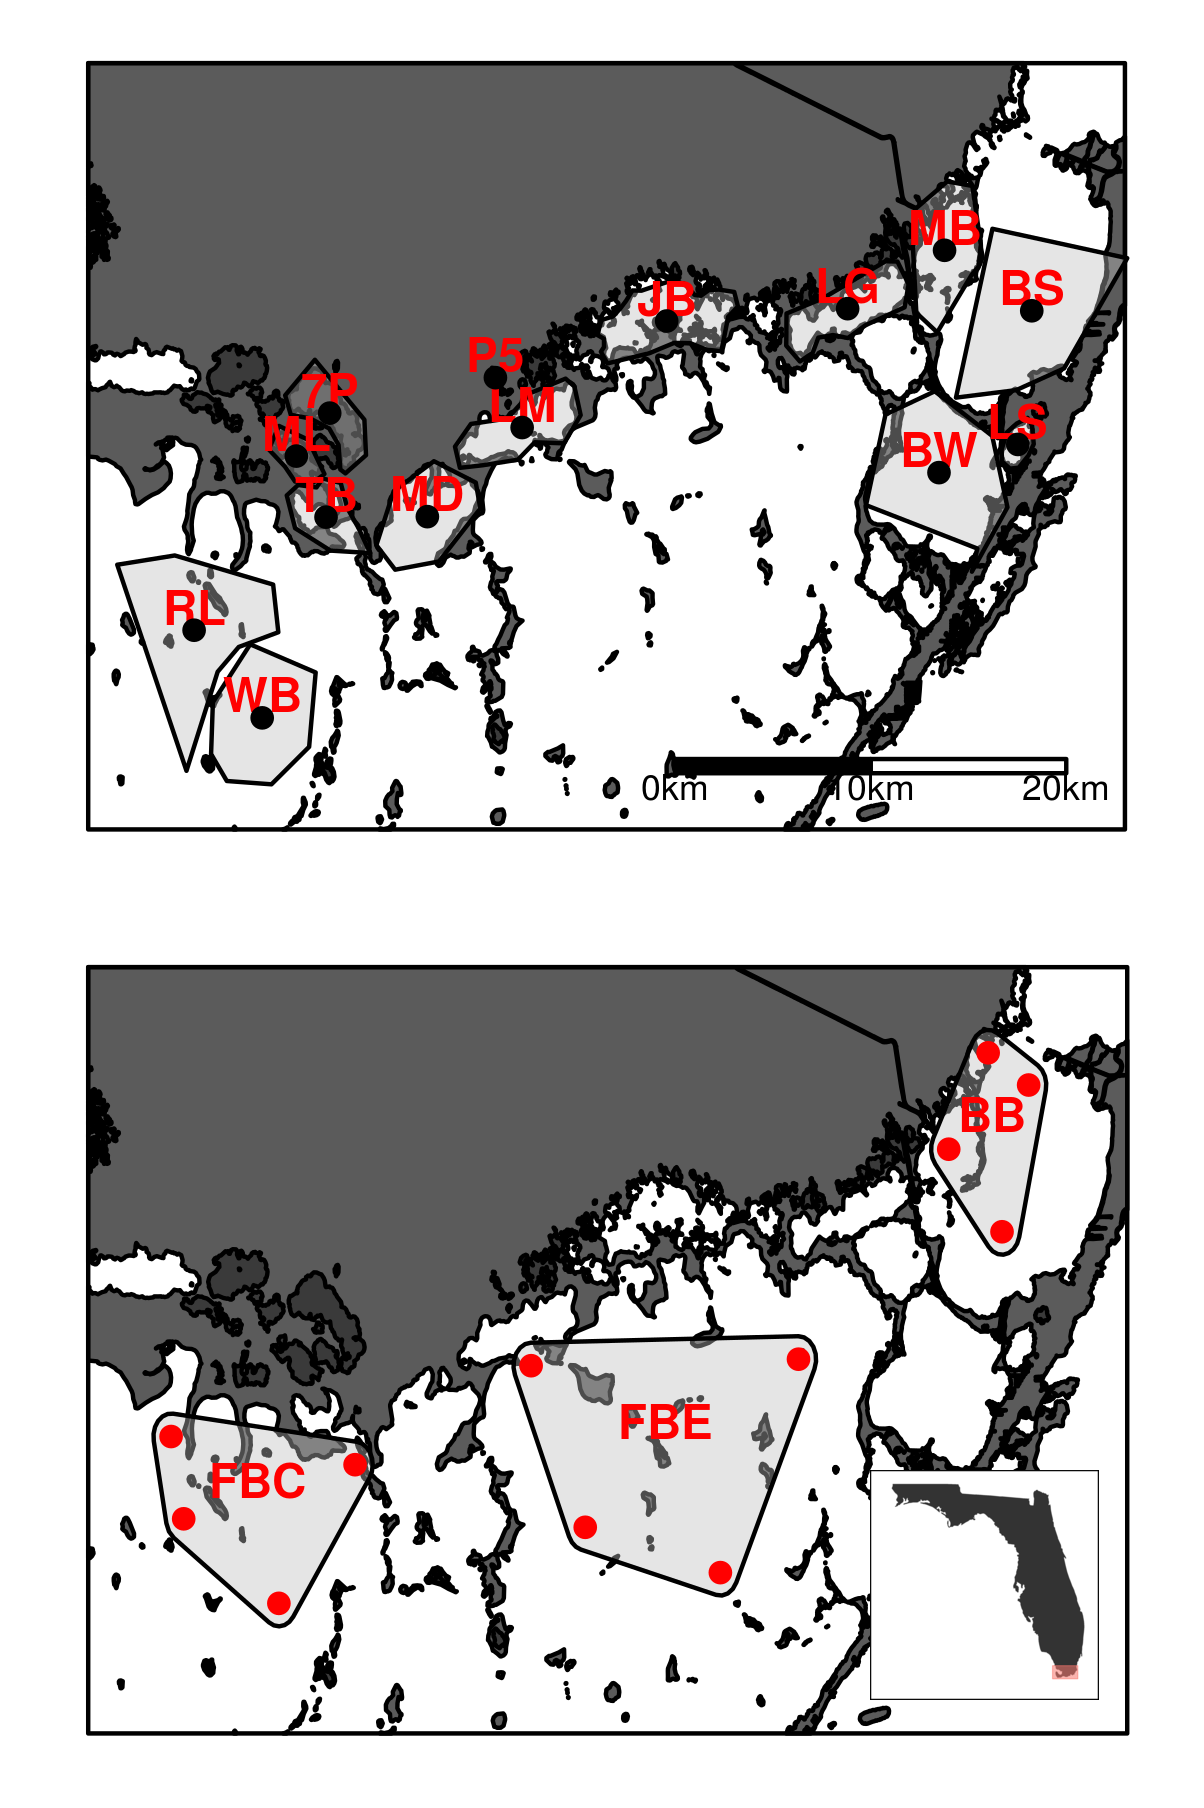
\includegraphics[width=0.75\textwidth]{../../figures/fbmap.png}
  \caption{Locations of discrete grab sampling sites within Florida Bay, USA. Polygons represent variability in sampling location over the course of the study period. Top: RL = Rankin Lake, WB = Whipray Basin, TB = Terrapin Bay, ML = Monroe Lake, 7P = Seven Palm Lake, MD = Madeira Bay, LM = Little Madeira Bay, P5 = Pond Five, JB = Joe Bay, LG = Long Sound, BW = Blackwater Sound, LS = Lake Surprise, MB = Manatee Bay, BS = Barnes Sound; Bottom: BB – Biscayne Bay, FBE – Florida Bay East, FBC = Florida Bay Central.}
  \label{fig:1}
\end{figure*}

\newpage

\begin{figure*}
  \centering
  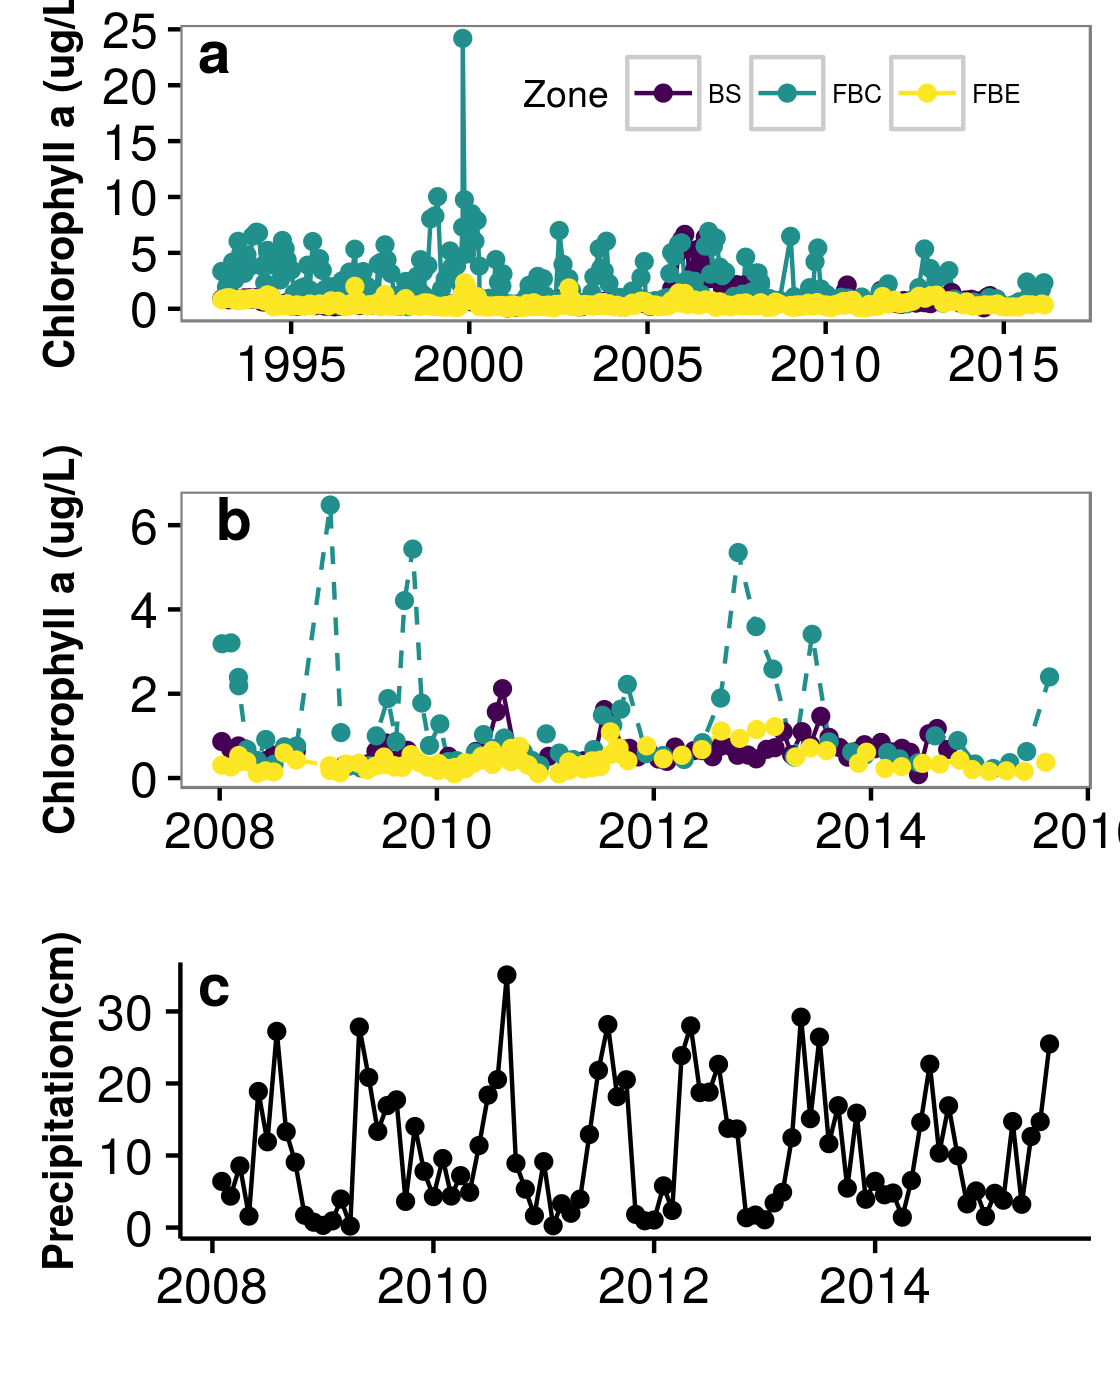
\includegraphics[width=0.75\textwidth]{../../figures/chltimeseries.png}
  \caption{Time series of average chlorophyll concentration within Florida Bay water quality zones. BS = Barnes Sound, FBC = Florida Bay Central, FBE = Florida Bay East. Precipitation during the study period. Precipitation data shown are composite means of three gages in the Florida Bay watershed.}
  \label{fig:2}
\end{figure*}

\newpage

\begin{figure*}
  \centering
  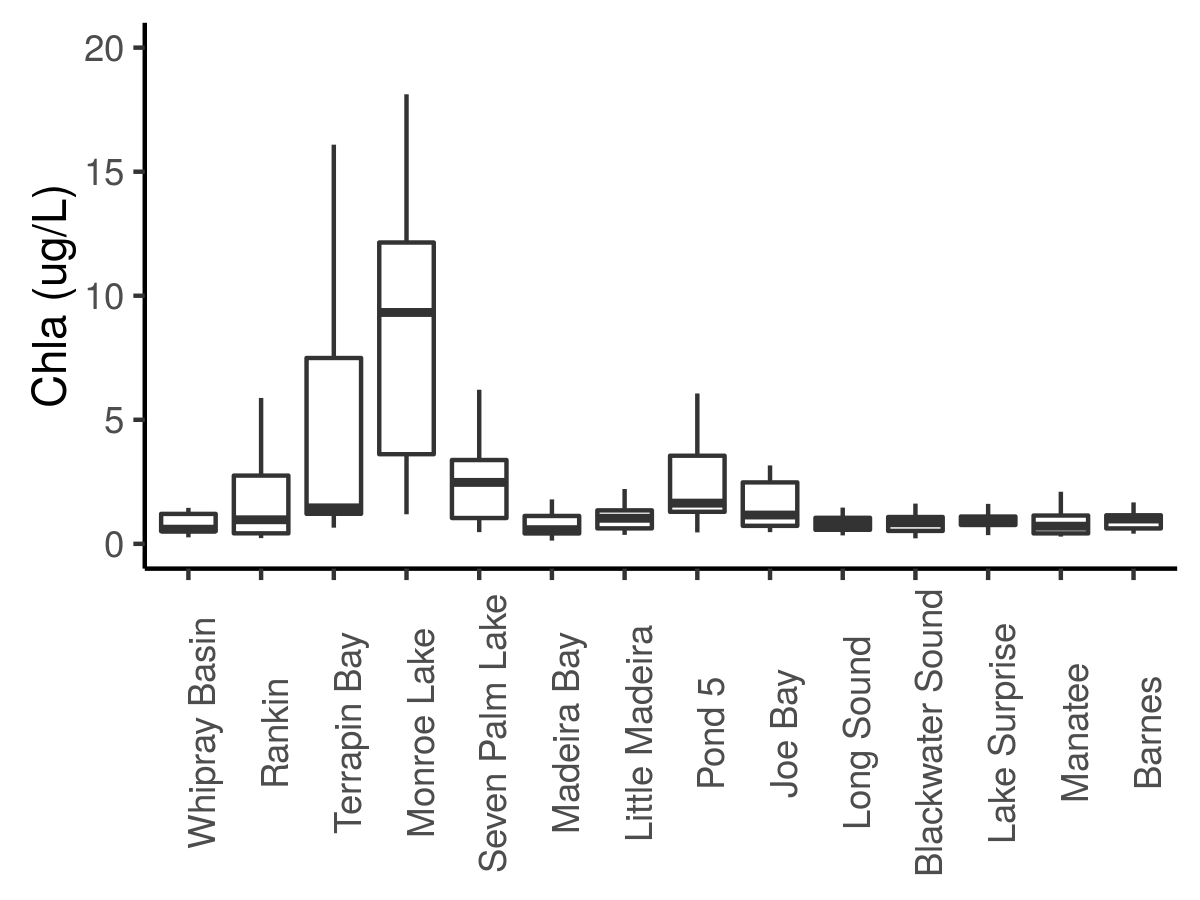
\includegraphics[width=0.75\textwidth]{../../figures/chlboxplot.png}
  \caption{Spatial distribution of chlorophyll concentration in selected Florida Bay basins. Basins are arranged geographically from west to east.}
  \label{fig:3}
\end{figure*}

\clearpage

\begin{figure*}
  \centering
  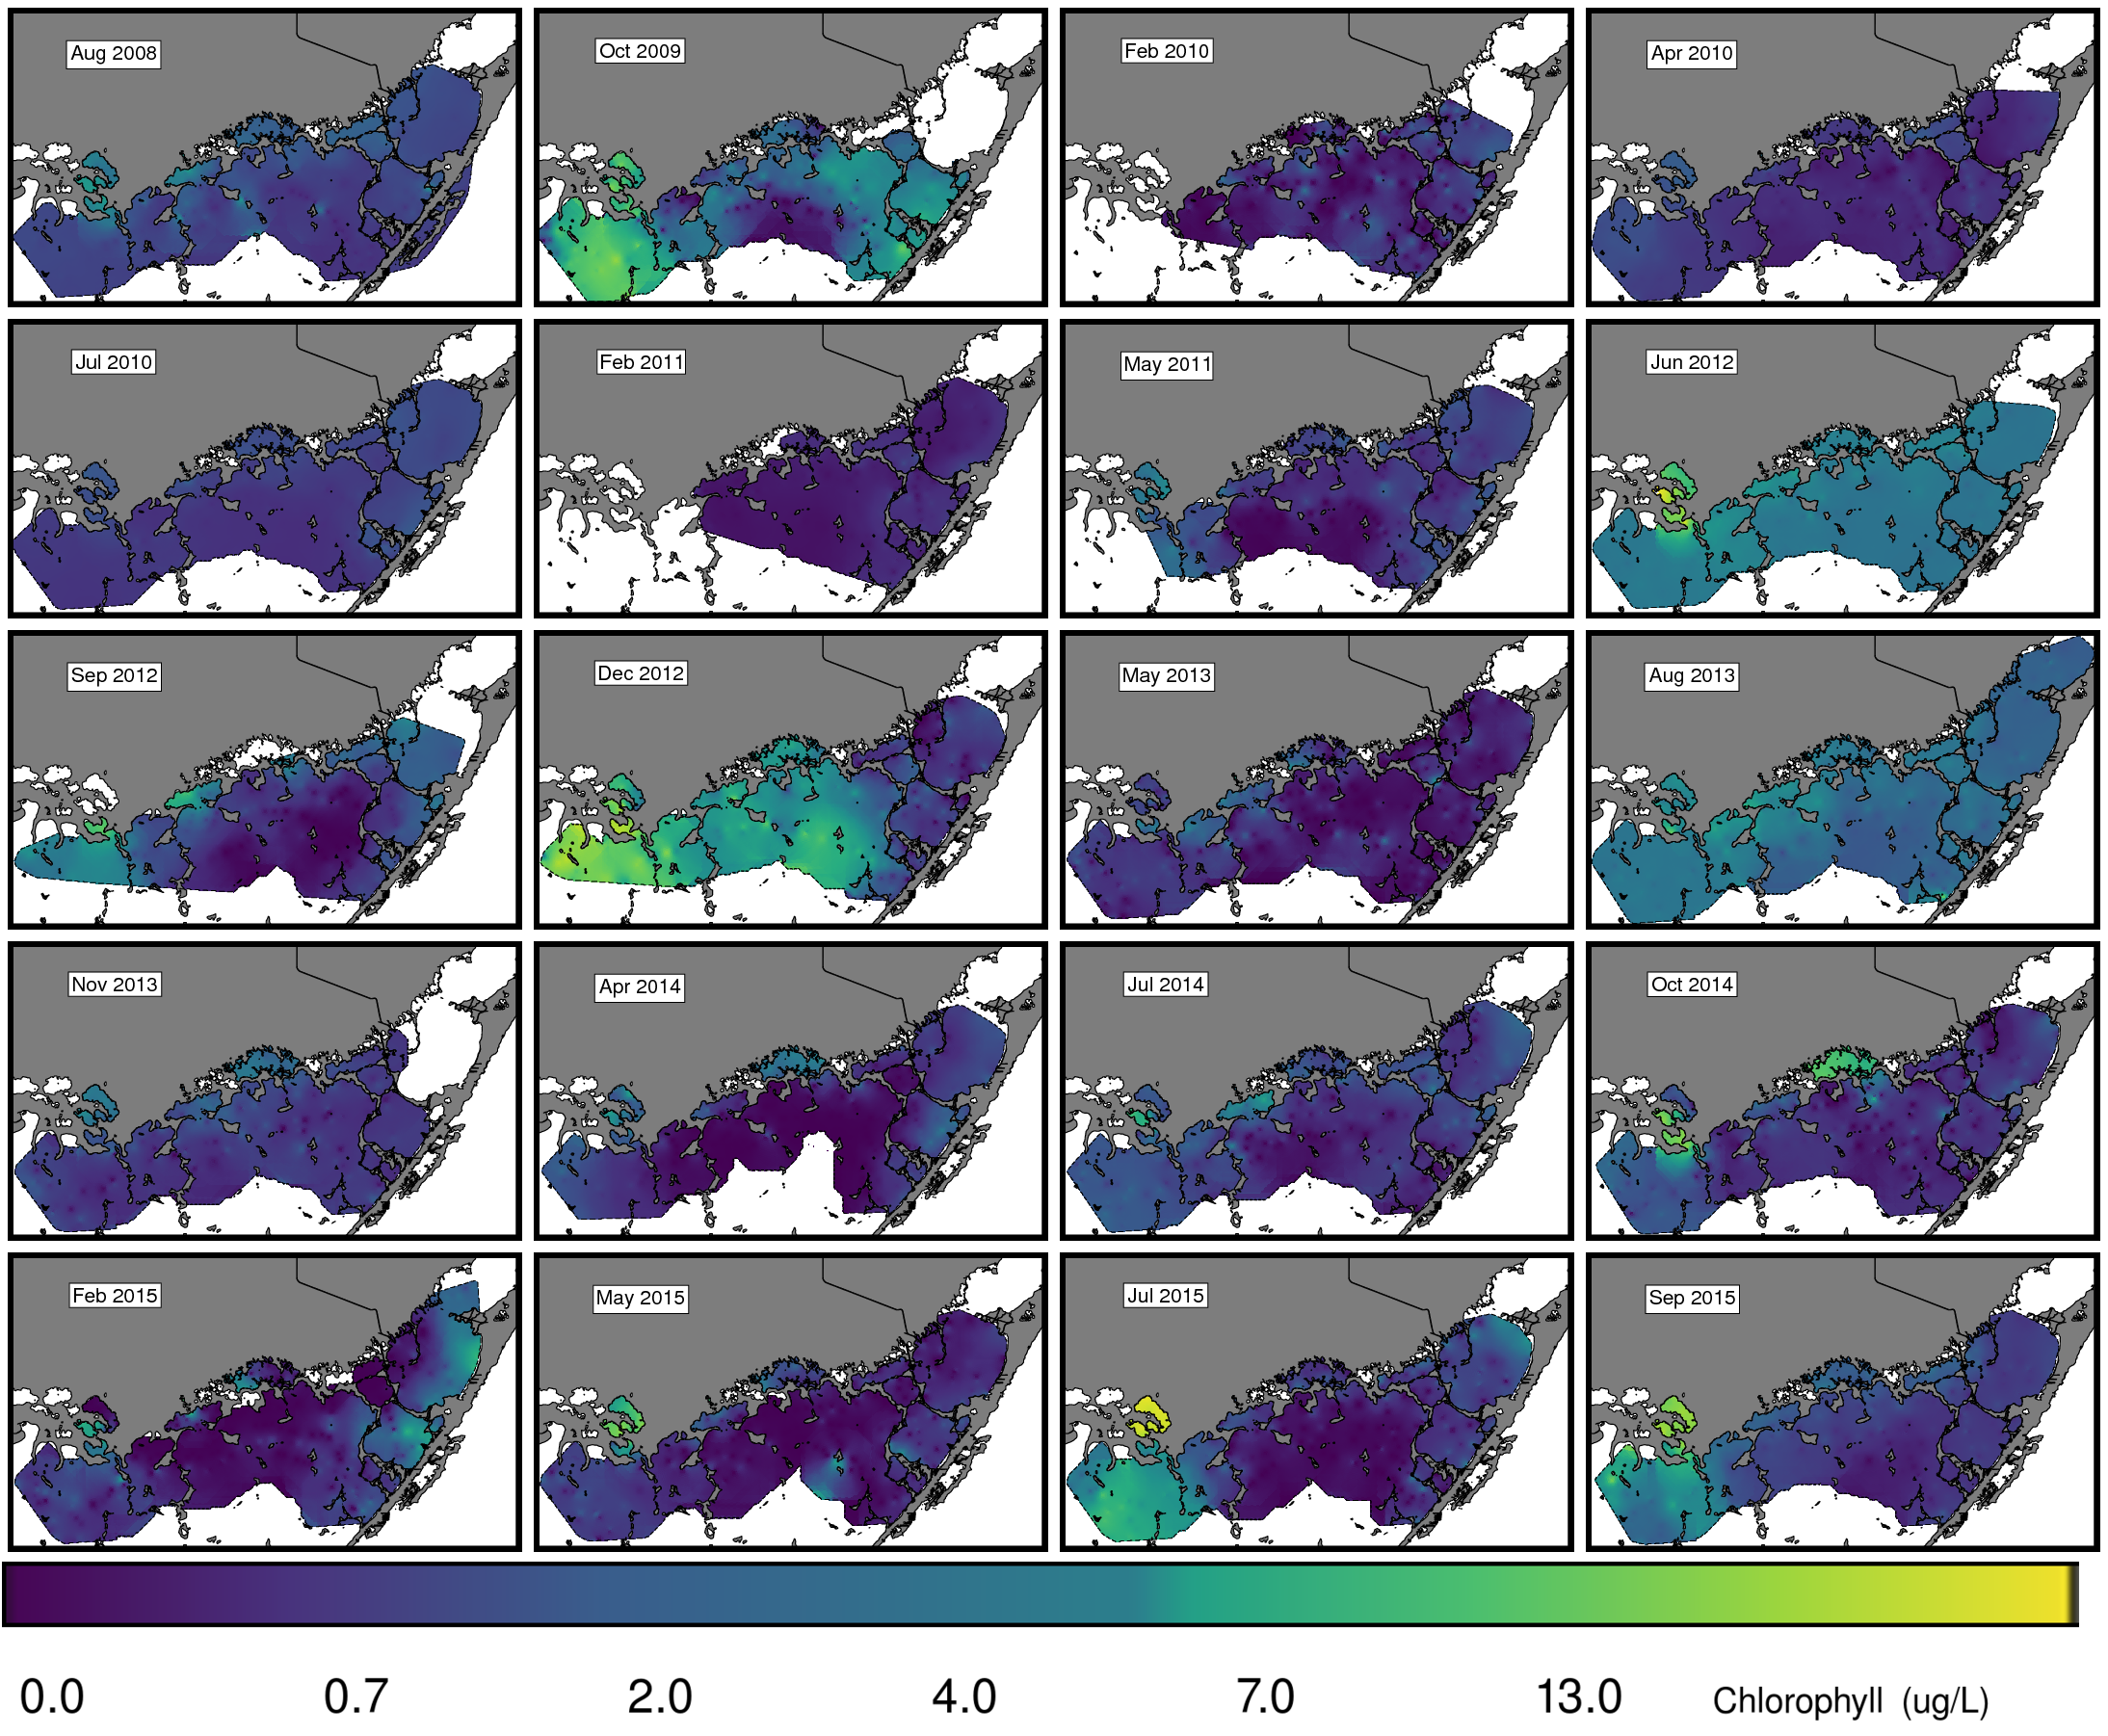
\includegraphics[width=0.75\textwidth]{../../figures/multipanel.png}
  \caption{Chlorophyll concentration calculated using the coefficients in Table 2. Note that the color ramp is log-scaled.}
  \label{fig:4}
\end{figure*}

\clearpage

\begin{table}
\centering
% library(xtable)
% dt <- read.csv("tables/grabs_cor.csv")
% dt <- dt[c(1, 2, 3, 6, 7), c(1, 2, 3, 6, 7)]
% xtable(dt)
% table caption is above the table
\caption{Correlation matrix of water quality parameters for selected Florida Bay basins. TP = total phosphorus, TDP = total dissolved phosphorus, PO4 = ortho-phosphate, TN = total nitrogen, chla = chlorophyll a, PP = particulate phosphorus. $**$ indicates a significant correlation at P $<$ 0.001}
\label{tab:1}       % Give a unique label
% For LaTeX tables use
\begin{tabular}{llllll}
\hline\noalign{\smallskip}
& tp & tdp & po4 & tn & chla \\
\noalign{\smallskip}\hline\noalign{\smallskip}
pp & 0.68** & 0.20 & 0.34 & 0.78** & 0.90** \\ 
tp  &  & 0.65** & 0.51** & 0.51** & 0.74** \\ 
tdp  &  &  & 0.48** & 0.09 & 0.28 \\ 
po4  &  &  &  & 0.97** & 0.63** \\ 
tn  &  &  &  &  & 0.67** \\ 
\noalign{\smallskip}\hline
\end{tabular}
\end{table}

\clearpage

\begin{figure*}
  \centering
  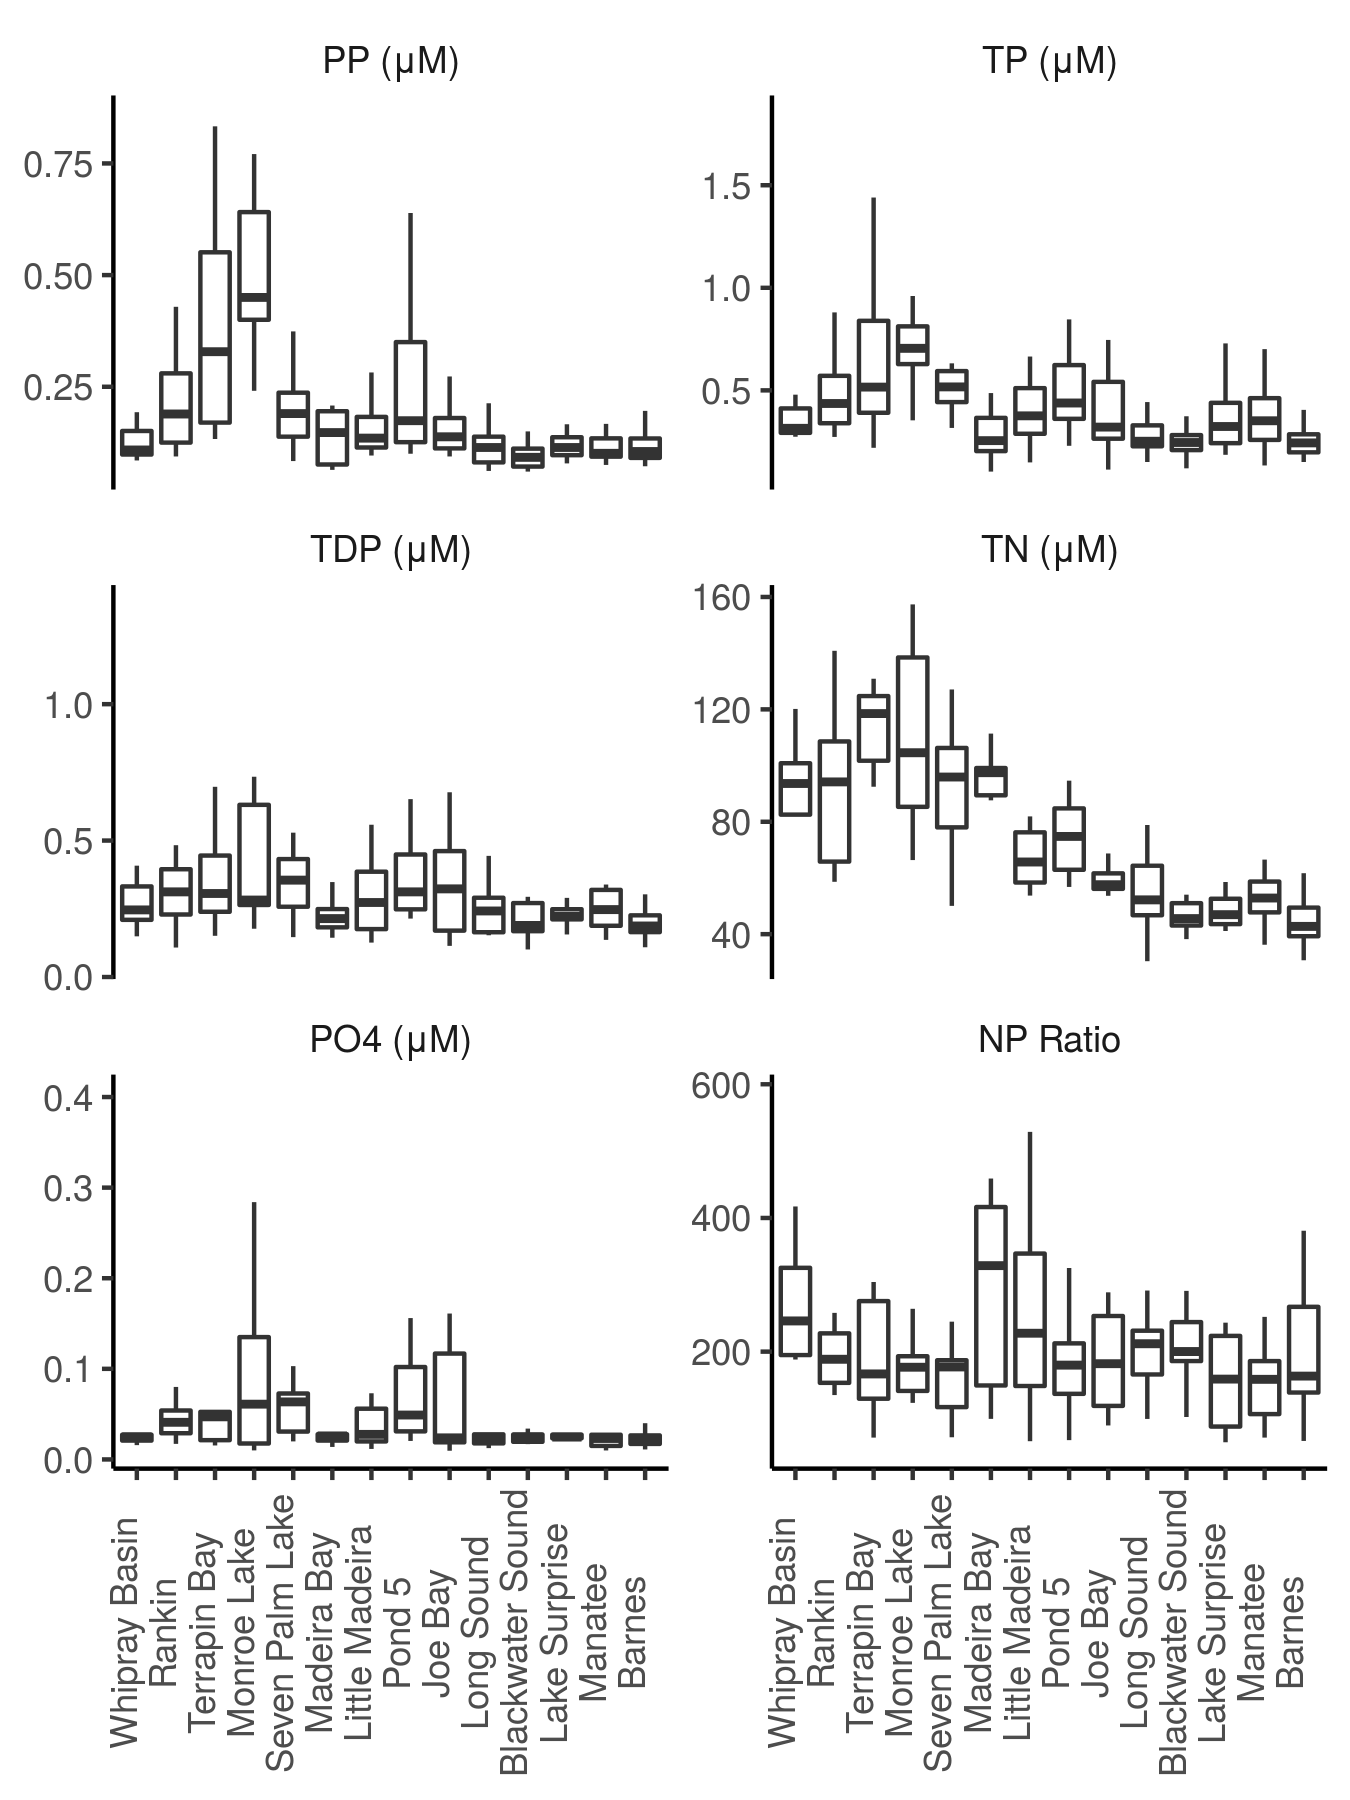
\includegraphics[width=0.75\textwidth]{../../figures/nonchlboxplot.png}
  \caption{Spatial distribution of discrete water quality parameters in selected Florida Bay basins.}
  \label{fig:5}
\end{figure*}

\newpage

\begin{table}
% library(xtable)
% dt <- read.csv("tables/modelfits.csv")
% dt <- dt[,c(2, 5:10, 17:19)]
% dt <- dt[order(dt$yearmon),]
% dt$pvalue <- round(dt$pvalue, 2)
% dt[dt$pvalue < 0.01 & !is.na(dt$pvalue), "pvalue"] <- "<0.01"
% print(xtable(dt), include.rownames = FALSE)
% table caption is above the table
\caption{Model coefficients for regressions between Dataflow and chlorophyll concentration of discrete grab samples. Also given is the coefficient of determination (R2) and p-value of each regression.}
\label{tab:2}       % Give a unique label
% For LaTeX tables use
\begin{tabular}{rrrrrrrrrr}
\hline\noalign{\smallskip}
date & cdom & chlaiv & phycoe & c6chl & c6cdom & phycoc & intercept & rsquared & pvalue \\ 
\noalign{\smallskip}\hline\noalign{\smallskip}
 2008-04 &  & 27.63 &  &  &  &  & -4.63 & 0.37 & 0.2 \\ 
  2008-08 &  & 5.12 &  &  &  &  & -0.14 & 0.90 & $<$0.01 \\ 
  2008-12 &  &  &  &  &  & 0.05 & 0.03 & 0.39 & 0.19 \\ 
  2009-04 &  &  &  &  &  &  &  &  &  \\ 
  2009-06 &  &  &  &  &  &  &  &  &  \\ 
  2009-10 & -67.15 &  &  & 0.05 &  &  & 6.27 & 0.97 & $<$0.01 \\ 
  2010-02 &  &  & 0.02 & 0.03 & -0.00 & -0.95 & 3.95 & 0.99 & 0.13 \\ 
  2010-04 &  & 7.83 &  &  &  &  & -0.92 & 0.69 & $<$0.01 \\ 
  2010-07 &  & 3.56 &  &  &  &  & 0.05 & 0.45 & 0.02 \\ 
  2011-02 &  &  &  & 0.01 & -0.00 &  & 0.00 & 0.98 & $<$0.01 \\ 
  2011-05 &  & 12.52 &  &  &  & 0.15 & -3.13 & 0.90 & $<$0.01 \\ 
  2011-06 &  &  &  &  &  &  &  &  &  \\ 
  2011-09 &  &  &  &  &  &  &  &  &  \\ 
  2012-03 &  &  &  &  &  &  &  &  &  \\ 
  2012-06 &  &  &  &  &  & 0.06 & 0.25 & 0.84 & $<$0.01 \\ 
  2012-09 &  & 20.29 &  &  &  &  & -3.43 & 0.84 & $<$0.01 \\ 
  2012-12 &  &  &  &  & 0.00 & 0.14 & -1.21 & 0.97 & $<$0.01 \\ 
  2013-04 &  &  &  &  &  &  &  &  &  \\ 
  2013-05 &  &  &  &  &  & 0.26 & -2.77 & 0.96 & $<$0.01 \\ 
  2013-08 &  &  &  &  &  & 0.16 & -0.26 & 0.68 & $<$0.01 \\ 
  2013-11 &  &  &  &  &  & 0.19 & -1.46 & 0.93 & $<$0.01 \\ 
  2014-02 &  &  &  &  &  &  &  &  &  \\ 
  2014-04 &  &  &  & 0.02 &  &  & -1.36 & 0.97 & $<$0.01 \\ 
  2014-07 &  &  & 0.00 & 0.00 &  & 0.15 & -2.62 & 0.91 & $<$0.01 \\ 
  2014-10 &  &  & -0.00 &  & -0.00 & 0.26 & -2.10 & 0.99 & $<$0.01 \\ 
  2015-02 &  &  &  & 0.01 & -0.00 & 0.05 & -0.97 & 0.94 & $<$0.01 \\ 
  2015-05 &  &  &  &  &  & 0.27 & -3.02 & 0.74 & $<$0.01 \\ 
  2015-07 &  & 0.81 &  &  &  & 0.32 & -5.74 & 0.98 & $<$0.01 \\ 
  2015-09 &  &  &  &  &  & 0.12 & -0.80 & 0.68 & $<$0.01 \\  
   \hline
% \noalign{\smallskip}\hline
\end{tabular}
\end{table}



\begin{figure*}
  \centering
  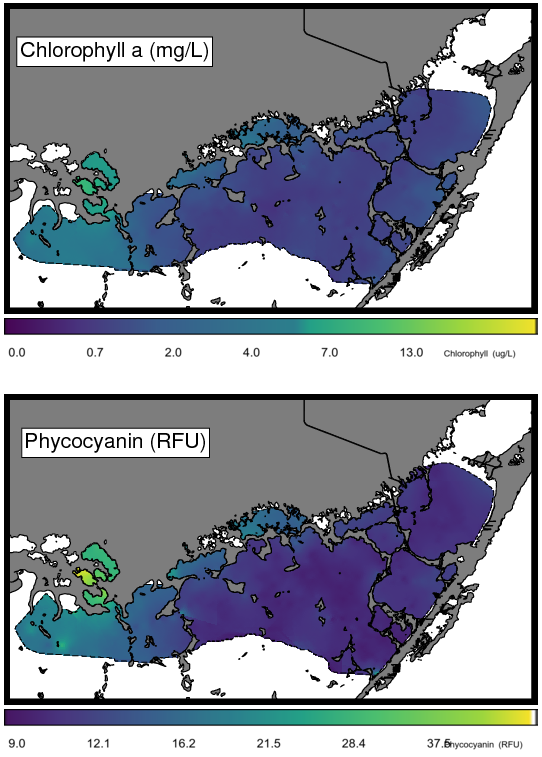
\includegraphics[width=0.45\textwidth]{../../figures/avmap.png}
  \caption{Maps of average chlorophyll a concentration and phycocyanin fluorescence.}
  \label{fig:6}
\end{figure*}

\end{document}
% end of file template.tex

